\documentclass{article}
\setlength{\parskip}{2.0mm}

\usepackage[hmargin=1.5cm,vmargin=1.5cm]{geometry}
\usepackage{listings}
\usepackage{color}
\usepackage{graphicx}
\usepackage{float}
\usepackage{amsmath}
\usepackage{subfig}
\usepackage{cite}
\usepackage{url}
\usepackage{amsmath}

\begin{document}

\title{3d Graphics - The sea seen from the beach}

\author{Jander Nascimento, 
\and Oleg Iegorov}

\maketitle

\section{Question 1}

\emph{Explain why rendering such a scene is very likely to produce
aliasing effects. Will the deformation of the sea surface due to waves
increase or tend to hide these visual problems?}

The aliasing effect happens when we try to render a high resolution image\cite{iaow}. Due to the render limitation we cannot represent the details of image in long distances. To overcome this issue a sampling is performed. As sampling selects certain pixels for displaying, the representation becomes inaccurate. The proper rendering of long distance pixels should be a composition (interpolation) of its neighbors.

In the Figure \ref{fig:aliasing} shows one example of aliasing effect in long distances representation (spatial aliasing).

\begin{figure}[H]
		  \centering
		  \subfloat[Sampled image]{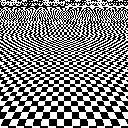
\includegraphics[width=0.4\textwidth]{image/alias01.png}\label{fig:sampled}}
		  \hspace{0.1cm}
		  \subfloat[Anti-aliased image]{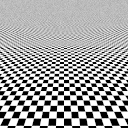
\includegraphics[width=0.4\textwidth]{image/alias02.png}\label{fig:antialiased}}
		  \caption{Aliasing effect}
		  \label{fig:aliasing}
\end{figure}

In the Figure \ref{fig:aliasing}, we are using a chessboard pattern as the texture for the ground. On the right handside we can see: the further the square is the more it acquires an incorrect shape. In the \ref{fig:antialiased} it is possible to see the result of an interpolation as anti-aliasing technique.	

An example with waves may reduce the aliasing effect due to the pseudo-random representation of the sea surface. The aliasing cannot be easily detected since the waves format is not strictly a regular pattern.


\section{Question 2}

\emph{A first idea for modeling the sea surface is to represent it by an
initially flat mesh, whose vertices will be displaced on the vertical
axis using z=Height(x,y,t). Two possible flat quadrangular meshes are
considered: a regular 2D grid and a grid computed by projecting the
pixels of the screen onto the horizontal plane of the sea, along the
viewing direction (so the mesh changes each time the camera moves).
Which of these representations would you use and why?}\\

The second variant of a grid is more efficient and produces better
results than a regular 2D grid. The reasons for that are the following\cite{iaow}:

\begin{itemize}

  \item We can move a camera over the sea surface maintaining an
    adequate resolution. As the grid is recalculated with each movement of
    the camera, zooming in and out is now possible with an acceptable
    resolution. Moreover, the waves animation hides the shift of sampling
    locations (which are the vertices of the projected quads).

  \item A concentration on the particular part of the sea is now
    possible. By increasing the number of the projected quads in
    the bottom of the screen we can add details in the foreground of the
    scene. At the same time, the reduced number of quads on the top of
    the screen says that we don't care much about the scene details
    near the horizon.

  \item Since the resolution depends on the size of the screen's quads,
    the waves that are smaller than the quads are not displayed. This
    fact increases performance reducing the computational time, as we
    work with smaller number of sampling locations.

\end{itemize}

As a result of using a dynamically recomputed grid, the number of
displayed waves is constant, since the more waves will be displayed in the
area of interest, and less --- in the neglected area. This fact, plus the
maintenance of an adequate resolution while moving a camera make such
technique preferable over a regular 2D grid.

\section{Question 3}

\emph{Another idea is to directly render the sea surface from the
procedural equation of its geometry Sea(x,y,t) = (x, y, Height(x,y,t)).
Which algorithm would you use? Explain the computations involved on a
figure. Can you adapt this algorithm to model specular reflections while
getting real-time performances?}

Assuming that we do not have a powerful machine to render the sea
surface at each timestep, the ray-tracing algorithm is not
suitable, as it requires a lot of CPU computations. Hence, we will
consider a texture mapping algorithm to render the sea surface as a less
costly alternative to ray-tracing. Having a texture map of the sea
surface and a procedural equation of its geometry, the mapping from
object coordinates to texture map coordinated is fairly simple. 

As a particular algorithm for rendering our scene we have chosen the Fresnel
Texture Mapping algorithm\cite{fresnel}. This algorithm is based on the Fresnel's law
of reflection which states that when the ray of light strikes the
sea surface at the angle less than 90 degrees, it is refracted as well
as reflected. Knowing this fact now we have to store two texture maps:
one for reflective information and the other for refractive information.
As the Fresnel's law states, the percentage of light reflected from the
surface is:

\begin{equation}
  I = \frac{sin^2(i-r))}{2sin^2(i+r)} + \frac{tan^2(i-r)}{2tan^2(i+r)}
\end{equation}

According to this algorithm a line is drawn between the camera and each
vertex to be rendered. Snell's law gives us the angles of
reflection ($\Theta_1$) and refraction($\Theta_2$): 

\begin{equation}
  \frac{sin\Theta_1}{sin\Theta_2} = \frac{v_1}{v_2}
\end{equation}

Substitution of this values into the Fresnel's formula gives us the
percentage of light reflected from the water. We can now use this
percentage to put weights into the reflective texture map information
(refractive and refractive texture maps information). Thus, the color
information for the point can be written as:

\begin{equation}
  (R_f,G_f,B_f) = I\cdot(R_{refl},G_{refl},B_{refl}) +
  (1-I)\cdot(R_{refr},G_{refr},B_{refr})
\end{equation}

Where $(R_f,G_f,B_f)$ is the final color triplet,
$(R_{refl},G_{refl},B_{refl})$ is the color triplet from the reflective
texture map and $(R_{refr},G_{refr},B_{refr})$ --- from the refractive
texture map. 

\section{Question 4}

\emph{The sea model is to be enhanced with some white foam: to simplify
the problem, we suppose that foam is projected forwards from the crest
of the waves at a given distance from the sea shore, falls onto the
water surface and then moves with it for a while before disappearing.
How would you animate and render the foam? Give the animation model
would you use, and describe the geometric primitive or the texture it
should control, and discuss its rendering.}

The foam creation can be achieved using the procedure-based modeling, following the two steps: choose a geometric primitive that generates foam, and use a technique for the foam dynamics.

The easiest way to render foam is to use spheres, changing the collision
algorithm, so they can be displayed overlapped. The next step is to create foam
texture, apply it to the spheres, and place it over a certain height,
introducing the volume aspect.  Although this looks unrealistic since if 
transparency is added to the foam, the intersections between spheres are not natural. 

Another alternative method to render foam is to use the Boundary Integral Method (BIM) to simulate foam dynamics\cite{bim}. The figure \ref{fig:dim-foam} shows an example of foam which was generated by this method.

\begin{figure}[H] \centering
  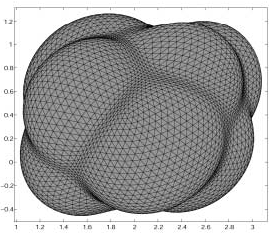
\includegraphics[width=0.4\textwidth]{image/dim01.png} \caption{Foam
  rendered by Boundary Integral Method} \label{fig:dim-foam}
\end{figure}

Transparency is an important aspect of the foam. It can be calculated\cite{nvidia} according to the equation
\ref{equa:transparency}, and applied to the geometric
primitive used for the foam representation.

\begin{equation} alpha=saturate(\frac{H-H_0}{H_{max} - H_0})
  \label{equa:transparency} \end{equation}

We can combine the texture with the BIM modeling the foam. We apply
the texture for the further visualization. Since the human eyes sees an interpolation
between the colors in the long distances, it is possible to apply the
texture for saving computation and reduce the aliasing effect.  For a
detailed visualization we render the geometric primitive with
BIM for the foam.

The dynamic aspect of the foam can be modeled using physically based animation. The particle should behave in respect to the gravity, and wind forces till the shore. The elevation of the waves crest defines the speed of the foam. It is possible to use the Gestner's model, as in this model we are aware of the wave trajectory. We can follow trajectory and set the very same path for the foam, applying some dispersion to it\cite{iaow}.
The environment conditions for the foam is that the waves must be sufficiently high enough to break and produce the foam(slope greater than 1/6 \cite{sow} of the height of the wave).
When the foam reaches the beach, it should disappear. We can simulate the burst of the bubble by the wind, removing layer by layer starting from the top.


\begin{thebibliography}{9}

  \bibitem{sow}
    Simulating Ocean Water,
    TESSENDORF, Jerry.
    2001

  \bibitem{fresnel}
    Modeling and Rendering Waves: Wave-Tracing using Beta-Splines and Reflective and Refractive Texture Mapping,
    PAULINE Y. TS'O and BRIAN A. BARSKY.
    University of California, Berkeley.
    1987.

  \bibitem{iaow}
    Interactive Animation of Ocean Waves,
    HINSINGER, Damien. NEYRET, Fabrice. CANI, Marie-Paule.
    iMAGIS-GRAVIR

  \bibitem{nvidia}
    GPU Gems 2,
    Kryachko,Yuri.
    GPU Gems 2. 
    Second printing, April 2005.
    \url{http://http.developer.nvidia.com/GPUGems2/gpugems2_chapter18.html}

  \bibitem{bim}
    Boundary Integral for 3d Simulation of Foam Dynamics,
    Ivan B. Bazhlekov, Frans N. van de Vosse, and Han E.H. Meijer.
    Eindhoven University of Technology.

\end{thebibliography}



\end{document}


